\documentclass[openany]{book}
\usepackage{framed}
\usepackage[version=3]{mhchem}
\usepackage{graphicx}
\usepackage{csvsimple}
\usepackage{longtable}
\usepackage{enumitem}
\newlist{steps}{enumerate}{1}
\setlist[steps, 1]{label = Step \arabic*:}
\newlist{properties}{enumerate}{1}
\setlist[properties, 1]{label = Property \arabic*:}
\usepackage{listings}
\usepackage{color} %red, green, blue, yellow, cyan, magenta, black, white
\definecolor{mygreen}{RGB}{28,172,0} % color values Red, Green, Blue
\definecolor{mylilas}{RGB}{170,55,241}
\lstset{language=Matlab,%
    %basicstyle=\color{red},
    breaklines=true,%
    morekeywords={matlab2tikz},
    keywordstyle=\color{blue},%
    morekeywords=[2]{1}, keywordstyle=[2]{\color{black}},
    identifierstyle=\color{black},%
    stringstyle=\color{mylilas},
    commentstyle=\color{mygreen},%
    showstringspaces=false,%without this there will be a symbol in the places where there is a space
    numbers=left,%
    numberstyle={\tiny \color{black}},% size of the numbers
    numbersep=9pt, % this defines how far the numbers are from the text
    emph=[1]{for,end,break},emphstyle=[1]\color{red}, %some words to emphasise
    %emph=[2]{word1,word2}, emphstyle=[2]{style},    
}
\title{%
	MATH 376: Numerical Analysis \\
	\large  Final Project
	}
\author{Quan Vu}
\date{\today}

\begin{document}
	\maketitle
	\chapter{Introduction}
	\section{Structure of the book}
	This book is intended to consolidate the knowledge that I've gathered through my time in the course MATH376: Numerical Analysis at Colgate University. I dedicate a chapter before each project to explain some of the numerical methods employed in the project itself.
	\section{Acknowledgements}
	I would like to take this opportunity to thank professor Seo Gunog for organizing and teaching this class. All the knowledge that I have gathered in this book is due to her teaching and guidance inside and outside class. Being a computer science and mathematics double major, I was able to find a very meaningful connection between the two subjects through this course, and altogether it has been a wonderful journey.\\\\
	I would also like to take this opportunity to thank my fellow classmates, Kevin Wibisono and Ruoyu (Tony) Guo, for always being there to support me throughout this course.  
	\chapter{Root finding methods - Bisection}
	\section{Method explanation}
	Imagine that you have a dictionary, and you are trying to find a definition of a word. What would you likely do? I myself would open the dictionary, and look at the page that I opened. If the words in those page come before the word that I'm looking for, I try to find a page between that current page and the end. If not, I do the opposite and find a page between the beginning and the current page. I repeat the process until I find the desired page/word.\\\\
	The bisection method works by employing similar intuition. The assumption is that we have a function whose root we want to determine, and we know for a fact that the function changes sign around this root. Then by using 2 initial guesses, acting as the beginning and the end of the dictionary, we look for a potential root in the middle. If this is the root that we want, then we just return from the process. Otherwise, we update the boundary of our "dictionary", and repeat the process until we find a satisfiable answer.
	\section{Method formalization}
	\begin{steps}
		\item Rewrite the equation in the form ${f(x) = 0}$
		\item Plot the graph of the function to determine the rough estimation of the desired root.
		\item Choose initial guesses ${a}$ and ${b}$ around the root, such that the function changes sign around this interval, i.e ${f(a) \times f(b)<0}$
		\item Find the estimated root, ${x_i = \frac{a + b}{2}}$
		\item If ${f(x_i) = 0}$, we're done, and we can return. Otherwise depending on the sign of ${f(x_i)}$, we update ${a}$ and ${b}$ accordingly. If ${f(x_i)}$ has the same sign as ${f(a)}$, then ${a = x_i}$, else ${b = x_i)}$. Return to step 4.
	\end{steps}
	\section{Error discussion}
	We assume that our next estimation is the real solution. From such assumption, it's easy to see that we are dividing the error in half by every time we are making a new estimation. The upper bound for the bisection method is ${\frac{b - a}{2^(n+1)}}$ where n is the number of iteration.
	\chapter{Greenhouse gases and pH}
	\section{Abstract}
	This chapter aims at examining the relationship between the steady 	rise in atmospheric levels of several greenhouse gases and the pH of rainwater within the corresponding areas. In particular, this project looks at the annual levels of atmospheric carbon dioxide (\ce{CO2}) from the year 1959 to 2016 in Mauna Loa, Hawaii. By computing the pH of water using the given data, it can be shown that the pH of rainwater has decreased from 5.63 to 5.58 over the years, and the trend shows that the pH level will likely drop lower.
	
	\section{Introduction}
	
	\subsection{Background information}
	It is well documented that the atmospheric levels of several “greenhouse” gases have been increasing over the past 57 years. It is also know that within areas with generally low human activities, carbon dioxide is the primary determinant of the pH of rainwater.
	
	\subsection{Problem description}
	This project aims at using the existing data regarding the levels of atmospheric \ce{CO2} around Mauna Loa to calculate the pH of rainwater in the same region over the years. This can be done with the help of five equations governing the chemistry of rainwater:
	\[ K_1 = \frac{10^6[H^+][HCO_3^-]}{K_HCO_2} \tag{1} \]
	\[ K_2 = \frac{[H^+][CO_3^{-2}]}{[HCO_3^-]} \tag{2} \]
	\[ K_\omega = [H^+][OH^-] \tag{3} \]
	\[ c_T = \frac{K_HCO_2}{10^6} + [HCO_3^-] + [CO_3^{-2}] \tag{4} \]
	\[ 0 = [HCO_3^-] + 2[CO_3^{-2}] + [OH^-] - [H^+] \tag{5} \]
	where ${K_H}$ is Henry's constant, ${K_1}$, ${K_2}$ and ${K_\omega}$ are equilibrium coefficients. The five unknowns are ${c_T}$ = total inorganic carbon, ${HCO_3^-}$ = bicarbonate, ${[CO_3^{-2}]}$ = carbonate, ${[H^+]}$ = hydrogen ion, ${[OH^-]}$ = hydroxyl ion.
	One major assumption with this approach is that we fix \ce{CO2} as the sole factor contributing to the pH of rainwater. In reality, many other greenhouse gases can also contribute to the fluctuation of pH.

	\subsection{Outline}
	Given the values ${K_H  = 10^{-1.46}}$, ${ K_1 =  10^{-6.3}}$, ${ K_2 = 10^{-10.3}}$, ${ K_\omega = 10^{-14}}$ and the annual \ce{CO2}, we can reduce equation (5) to be one that is in terms of ${[H^+]}$. We can compute ${[H^+]}$ and calculate the pH of rainwater using the equation:
	\[ pH = -log_{10}[H^+] \tag{6} \]
	
	\section{Numerical method}
	Firstly we convert the given equations so that the unknowns in (5) can be expressed in terms of ${[H^+]}$. \\
	From (1):
	\[ [HCO_3^-] = \frac{K_HK_1CO_2}{10^6[H^+]} \tag{1a} \] \\
	From (2) and from (1a):
	\[ [CO_3^{-2}] = \frac{K_2[HCO_3^-]}{[H^+]} \tag{2a} = \frac{K_HK_1K_2CO_2}{10^6[H^+]^2} \] \\
	From (3):
	\[ [OH^-] = \frac{K_\omega}{[H^+]} \tag{3a} \] \\
	From (4), (2a) and (3a):
	\[ c_T = \frac{K_HCO_2}{10^6} + \frac{K_HK_1CO_2}{10^6[H^+]} + \frac{K_HK_1K_2CO_2}{10^6[H^+]^2} \tag{4a} \]
	From 5, and from (1a), (2a), (3a):
	\[ 0 =  \frac{K_HK_1CO_2 + 10^6K_\omega}{10^6[H^+]} + \frac{2K_HK_1K_2CO_2}{10^6[H^+]^2}] - [H^+] \tag{5a} \]
	By using the bisection method on the above equation, we can find ${[H^+]}$. \\
	A short snippet of Matlab code is attached in the appendix for this section to show how the bisection method finds the root of the function. 
	
	\section{Results}
	Using the methodology discussed above, we obtain the following results of the pH levels in rainwater in Mauna Loa, from 1959 to 2016:\\
	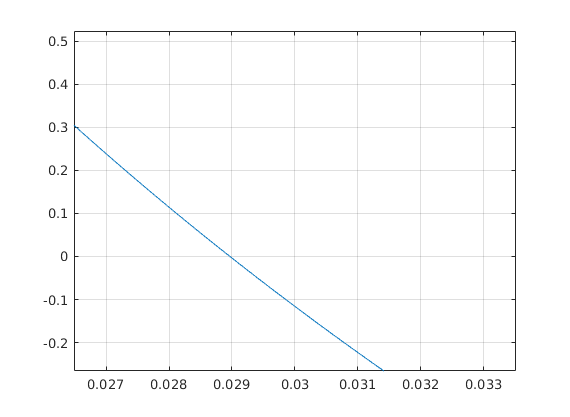
\includegraphics[scale=0.6]{untitled.jpg} \\
	For detailed results, consult the csv file in the project directory.
	
	\section{Discussion}
	From the calculations taken, the pH in the year 1959 was 5.63, and the pH calculated in 2016 was 5.58. While the decline seems small, we must keep in mind that pH is calculated by taking ${log_{10}}{[H^+]}$. This means that the concentration of Hydrogen ions in rainwater has increased over the year, and the trend does not seem to be stopping. In fact this trend can be modeled using the polyfit function in Matlab to give:
	\[pH = -5.523 \times 10^{-6}t^2 + 0.02101t - 14.33\] 
	where t denotes the year. If the trend continues, the pH of rainwater will drop below the threshold of 5.0, creating acid rain.\\\\
    An interesting observation is that pH seems to drop with the rise of \ce{CO2}. Such investigation can be carried out in further researches to find a direct relationship between these two. The total inorganic carbon was also not discussed within the scope of this project, but at the same time it might be interesting to look into this. Presumably, with the rise in \ce{CO2}, ${c_T}$ should rise as well, showing that there is an abundance in inorganic carbon intake.
	\section{Bibliography}
	Data for annual atmospheric levels of \ce{CO2} are taken from: \\
	https://www.esrl.noaa.gov/gmd/ccgg/trends/data.html
	\section{Appendix for this chapter}
	\subsection{Code for the bisection method}
	\lstinputlisting{bisectM.m}
	\subsection{Code for processing data}
	\lstinputlisting{Project1.m}
	\chapter{More root finding methods}
    \section{Introduction}
    The bisection method has its merits in the sense that we are always guaranteed to find an answer to the problem, given that our assumptions are correct. The downside is that it can be slow to converge, and that if the function does not change signs around the root, this method is not employable.\\
    In this section, we explore a few other root finding techniques, which are the method of false position, Newton's method and the method of fixed point iteration.
    \section{Method of false position}
    \subsection{Method explanation}
    The method of false position fixes the shortcoming of the bisection method. The method starts out with the same assumption as the bisection method. We need 2 initial guesses and also we assume that the function changes sign around the roots. The method estimates the root by assuming that the function is the straight line connecting the two points evaluated at the estimations, and find the root of that straight line. Depending on the sign of the function at the new estimation, we update the endpoints accordingly.
    \subsection{Method formalization}
    \begin{steps}
    	\item Rewrite the equation in the for ${f(x) = 0}$
        \item Plot the graph of the function to determine the rough estimation of the desired root.
		\item Choose initial guesses ${a}$ and ${b}$ around the root, such that the function changes sign around this interval, i.e ${f(a) \times f(b)<0}$
        \item Find the estimate of the root, determined by 
        \[x_i = a - f(a)\frac{b - a}{f(b) - f(a)}\]
        \item If ${f(x_i) = 0}$, we're done, and we can return. Otherwise depending on the sign of ${f(x_i)}$, we update ${a}$ and ${b}$ accordingly. If ${f(x_i)}$ has the same sign as ${f(a)}$, then ${a = x_i}$, else ${b = x_i)}$. Return to step 4.
    \end{steps}
    \subsection{Method discussion}
    The method of false position assures convergence if the function changes signs around the desired root. It may converge faster than the bisection method, since it assumes takes the value of the functions at the estimations into account, instead of just mindlessly assumes that the midpoint is a good estimation for the root.\\
    One problem with the false position method is that it may happen that all of the approximations lie on one side of the root, and therefore it converges very slowly for functions with significant curvature.
    \section{Newton's method}
    \subsection{Method explanation}
    Newton's method is the first method that we encounter that does not rely on having 2 estimations. By employing only one estimation at the beginning, we can iteratively find a better estimate for the solution. The method assumes that the function is linear, and as such the root of the tangent function at our estimate would give us the value of the actual root of the function. The value gets updated iteratively until the error is within tolerance.
    \subsection{Method formalization}
    \begin{steps}
    	\item Plot the graph of the function f.
        \item Start with an initial guess of a desired root, ${x_0}$, which is chosen from the graph of f
        \item Draw the tangent line to the curve ${y =f(x)}$ at the point ${(x_0), f(x_0)}$
        \item Find the x-intercept of the tangent line and label it ${x_1}$
        \[x_1 = x_0 - \frac{f(x_0)}{f'(x_0)}\]
        \item Repeat steps 3 and 4 by replacing the old estimation with the new estimation, until the error is within acceptance criteria
    \end{steps}
    \subsection{Method discussion}
    We have the following theorem;
    \paragraph{a} If ${x_R}$ is a simple root, convergence is quadratic (or second order), and ${|E_{n+1}| \approx \frac{|f''(x_R)|}{2|f'(x_R)|}|E_n|^2}$
    \paragraph{b} If ${x_R}$ is a multiple root of order k, convergence is linear and  ${|E_{n+1}| \approx \frac{k-1}{k}|E_n|}$
    \section{Fixed point iteration method}
    \subsection{Method explanation}
    The premise of this method based solely on whether we can represent the original equation ${f(x)}$ in the form ${g(x) = x}$. Then by employing an initial guess, we iteratively compute the value of ${g}$ at the guess, and that would give us an update on the estimation for the value of the root.
    \subsection{Method formalization}
    \begin{steps}
    	\item Find an iteration function ${g(x)}$ by rewriting ${f(x)}$ in the form ${x = g(x)}$
        \item Choose an initial approximation for the root, ${x_0}$
        \item Using the iteration formula, obtain ${x_1 = g(x_0)}$
        \item Repeat step 4 until we find a solution that false within tolerance
    \end{steps}
    \subsection{Method discussion}
    The method of fixed point iteration's beauty lies in its simplicity. However at the same time, the method is not guaranteed to converge. It is a possibility that the iteration function was chosen badly, and as such the approximations diverge away from the desired root.\\\\
    We have the following theorem: \\
    \noindent\fbox{%
    	\parbox{\textwidth}{%
    		Let ${g \in C[a,b]}$ be such that ${g(x) \in [a,b] \forall x \in [a,b]}$. Suppose that in addition, that ${g'}$ exists on ${(a,b)}$.Then the iterations are convergent on the interval ${[a,b]}$ if the interval contains a root and if ${|g'(x)| < 1 \forall x \in [a,b]}$
    	}%
    }
	\chapter{Fluid flows in pipes and tubes}
	\section{Abstract}
	This chapter aims at examining the flow of fluid through pipes and tubes. The project computes the dimensionless \textit{friction factor} in turbulent flows. By computing this factor using the bisection method, the false position method, Newton's method and lastly the fixed point iteration method, this paper draws out comparisons between how effective these methods are and what are the constraints associated with them.
	
	\section{Introduction}
	
	\subsection{Background information}
	Determining the friction factor is of great relevance to many field of engineering and science. Some of these include the flow of liquid and gases through pipelines and cooling systems. Scientists are interested in topics ranging from the flow in blood vessels to nutrient transmission through a plant's vascular system.
	
	\subsection{Problem description}
	In turbulent flows, the \textit{Colebrook equation} provides a means to calculate the friction factor using the equation\\
    \[ 0 =  \frac{1}{\sqrt{f}} + 2.0 \log_{10} \left(\frac{\varepsilon}{3.7D} + \frac{2.51}{\textit{Re}\sqrt{f}}\right) \] \\
    where $\varepsilon$ is the roughness (${m}$), D is the diameter (${m}$), and \textit{Re} is the Reynold's number, as calculated by
    \[\textit{Re} = \frac{\rho V D}{\mu}\]
    where $\rho$ is the fluid's density (${kg/m^{3}}$), V is the velocity (${m/s}$), and ${\mu}$ is the dynamic viscosity (${N.s/m^2}$)
    
	\subsection{Outline}
	By computing Reynold's number using the given values, we can substitute it back into the equation and using the numerical methods discussed, we can find the value of the friction factor. The given values are ${\rho = 1.23 kg/m^3}$, ${\mu = 1.79 \times 10^{-5} N.s/m^2}$, ${D = 0.005 m}$, ${V = 40 m/s}$, and ${\varepsilon = 0.0015 mm}$
	
	\section{Numerical methods}
	The numerical methods involved in the calculation of the friction factor are the bisection method, false position method, Newton's method, and fixed-point iteration method. Consult the attached Matlab project file to see the details of the calculations
	
	\section{Results}
	\subsection{Reynold's number}
    Using Matlab, we are able to determine Reynold's number = ${1.374 \times 10^4}$
    \subsection{Plotting graph and estimation}
    Using Matlab to plot the graph, the friction factor seems to be somewhere around 0.029 \\
    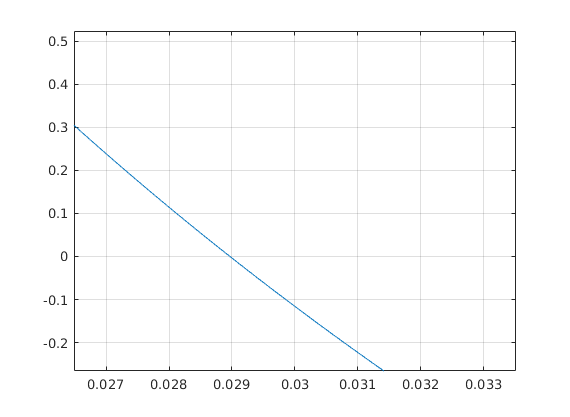
\includegraphics[scale=0.6]{untitled.png}
    
    \subsection{Bisection method and False position method}
    For both of these methods, we approximate the value of the friction factor by using a = 0.008 and b = 0.08, with a tolerance of ${10^{-8}}$
    \subsubsection{Bisection method}
    The method took 26 iterations to calculate the answer. The estimations converge to 0.02896781 
    \subsubsection{False position method}
    The method took 31 iterations to calculate the answer. The estimations converge to 0.02896782
    \subsubsection{Discussion}
    We see that both method converges to the solution, however the bisection method is faster in this case.
    \subsection{Newton's method}
    We can calculate the derivative of the function quite easily: \\
    \[ h'(f) = \frac{-1}{2 f \sqrt{f}} + 2.0 \left(\frac{log_{10} e \times \frac{-2.51}{2 \textit{Re} f \sqrt{f}}}{\frac{\varepsilon}{3.7D} + \frac{2.51}{\textit{Re}\sqrt{f}}}\right) \]\\
    This is then used for the calculation for Newton's method in the Matlab file provided in the appendix.
    \subsubsection{With initial guess 0.008}
    Took 6 iteration to calculate the answer. The estimations converge to 0.02896781 
    \subsubsection{With initial guess 0.08}
    The approximations do not converge. They fluctuate and eventually go to infinity
    \subsubsection{Discussion}
    We see that Newton's method converges extremely fast if we choose the correct initial guess. This is due to the nature of the function around the root.
    \subsection{Using fzero}
    We use the built-in fzero function with options = optimset('Display','iter', 'TolX', 1e-8).This function searches for a point near the guess where the sign of the function changes
    \subsubsection{With initial guess 0.008}
    The method does not converge to the solution. Complex function value encountered during search
    \subsubsection{With initial guess 0.08}
    The method manages to find an interval [0.0288, 0.116204] where the function changes sign. It then continues to search for the root by evaluating possible values in this interval, and eventually got to f = 0.0289678 
    \subsubsection{Discussion}
    As opposed to Newton's method, fzero was able to find the root with initial guess 0.08, but was unable to do so with initial guess 0.008.
    \subsection{Fixed Point Iteration}
    \subsubsection{Iteration function}
    The fixed point method relies on whether we can find an iteration function ${g(x)}$ such that ${f(x) = x - g(x)}$ and ${|g(xR)| < 1}$ where ${xR}$ is the root of the function. By repeatedly finding ${x}$ for which ${x = g(x)}$, a reasonable estimate for the root is found. The code illustrating this method is attached in the appendix.\\
    \\
    One of the possible iteration functions is: \\
    \[ g(f) = \left(\frac{1}{2.0 \log_{10} \left(\frac{\varepsilon}{3.7D} + \frac{2.51}{\textit{Re}\sqrt{f}}\right)}\right)^2 \]
    \subsubsection{Cobweb Diagrams}
    For initial guess f = 0.008: \\
    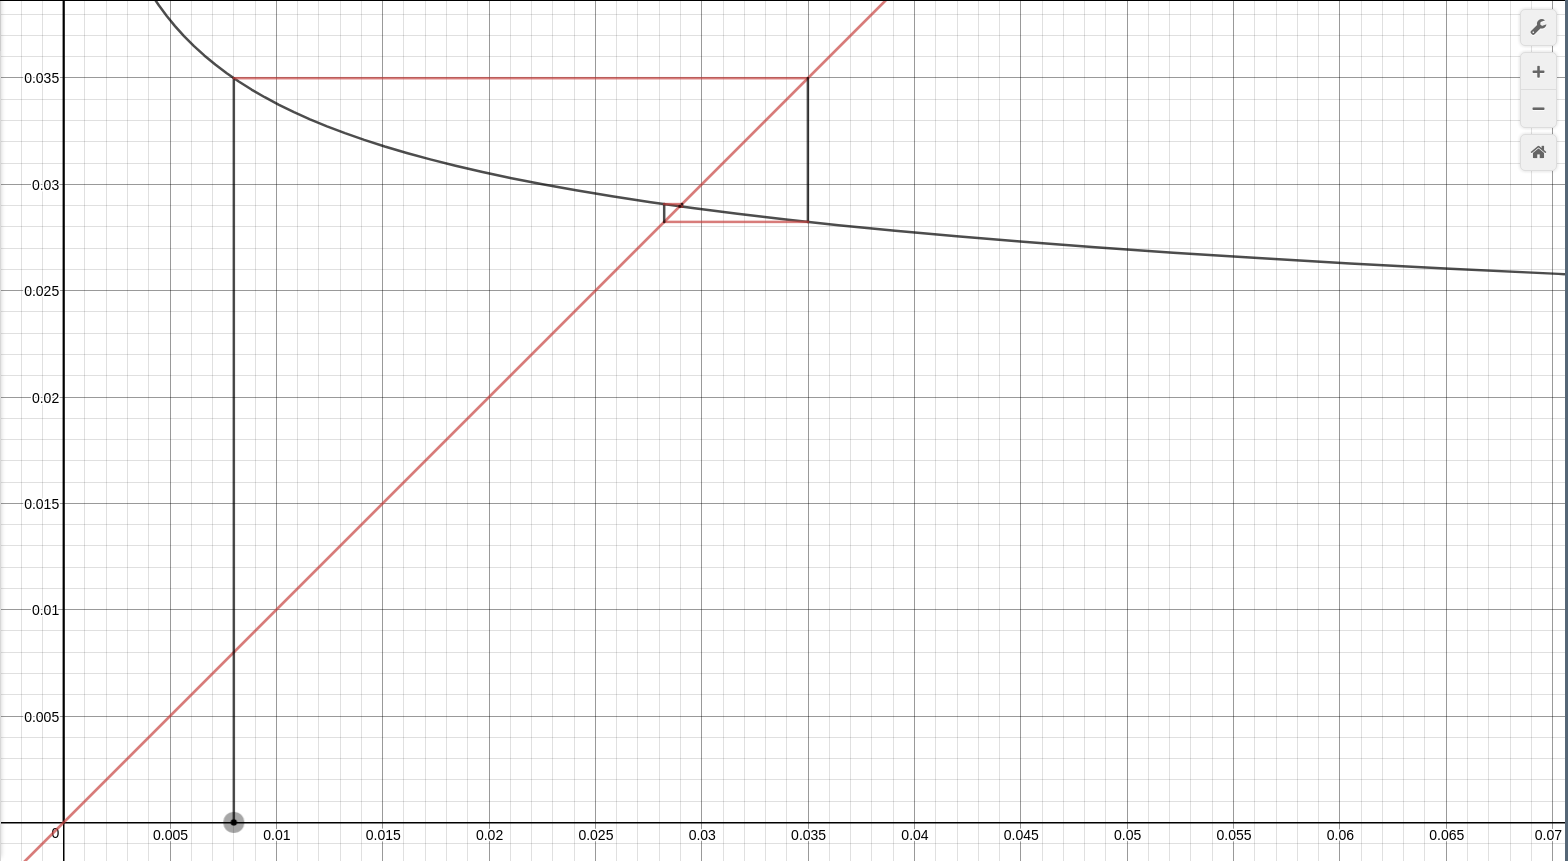
\includegraphics[scale=0.2]{second.png}\\
    For initial guess f = 0.08: \\
    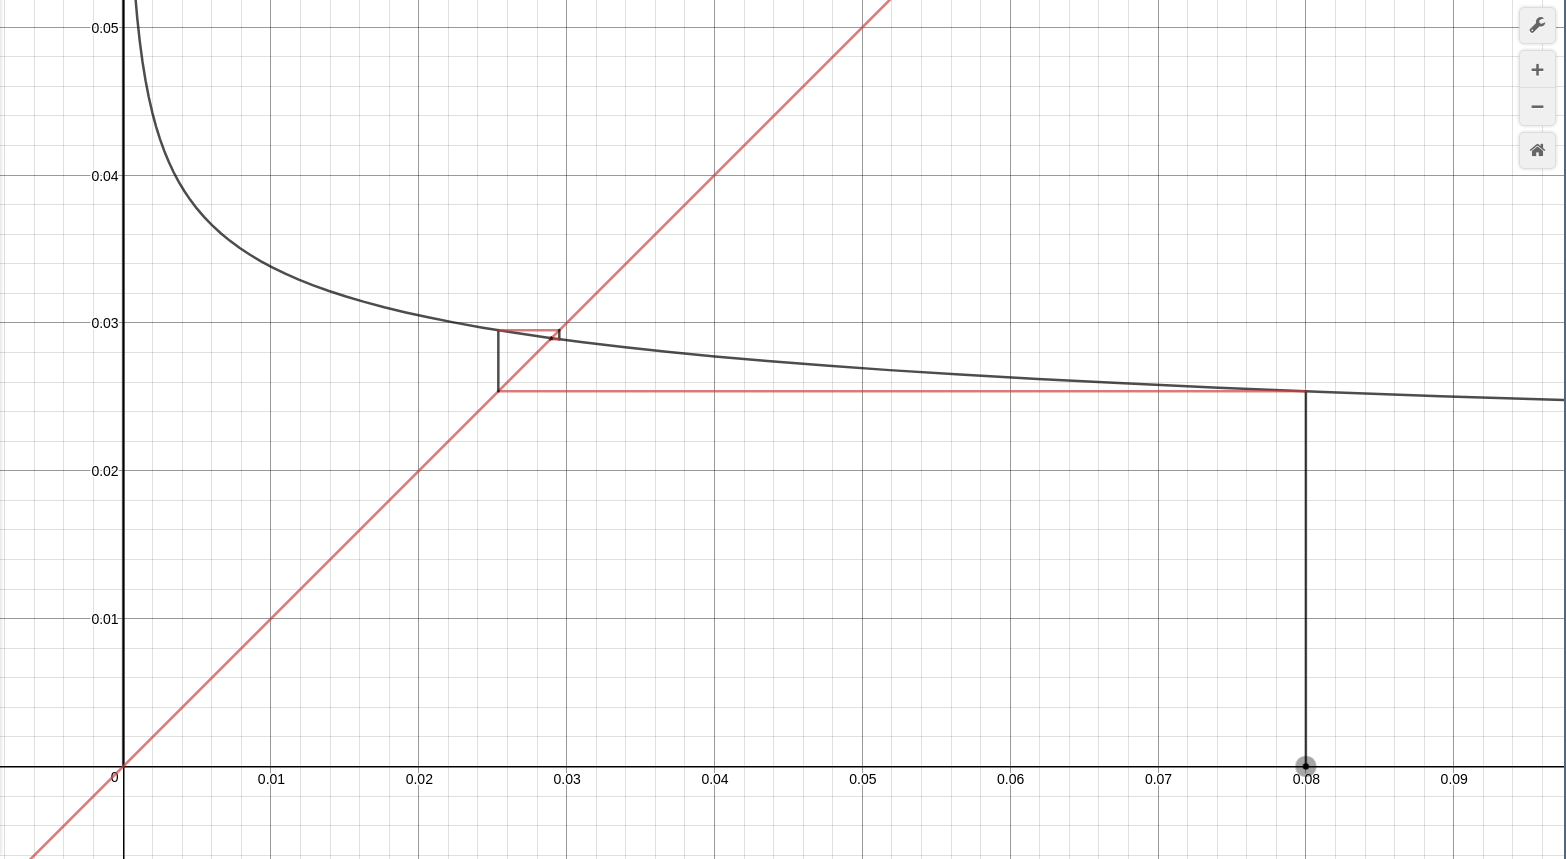
\includegraphics[scale=0.2]{first.png}\\
    \subsection{}{Discussion}
    With both initial guesses at 0.008 and 0.08, the method was able to find the approximation in 9 iterations. This is because ${|g'(x)| < 1}$ at the root and therefore guarantees convergence.
    \section{Consolidation of smaller discussions}
    We see that both the bisection method and the false position method were able to converge to the solution no matter what. This is unsurprising, since we know that the two methods are actually quite similar in nature. The bisection method converges faster, suggesting that there is some significant curvature to the equation that we are looking at.\\\\
    Newton's method converges extremely fast if we choose the correct initial guess, however it falls apart equally quickly if we don't. Further discussion can revolve around what are the conditions for Newton's method to guarantee convergence, and how it depends on certain functions and their respective behaviors around their roots.\\\\
    The method of fixed point iteration guarantees convergence due to the nature of the iteration function around the root. Further experimentation suggests that no matter what initial guess is used, the method will always find its way back to the root, further confirming our theorem stated in the previous chapter. Further discussion can involve finding a different iteration scheme to see if such scheme also guarantees convergence, and if it doesn't, why.
    
    \section{Appendix for this chapter}
    \subsection{Code for the false position method}
	\lstinputlisting{falsePositionM.m}
    \subsection{Code for Newton's method}
	\lstinputlisting{NewtonsM.m}
    \subsection{Code for fixed point method}
	\lstinputlisting{fixedpointM.m}
    \subsection{Code for this chapter}
	\lstinputlisting{Project2.m}
    
    \chapter{Solving systems of linear equations}
    \section{Introduction}
    So far we have explored several methods for solving for the root of a function. Now we make a little switch and look at systems of linear equation. Gaussian elimination is widely used to reduce matrices to forms that are easier to work with, thus enabling us to use backward substitution to solve for the solutions of the system. Another commonly used method is the LU factorization method, which is more efficient that traditional Gaussian elimination since it can be done independently of the constant matrix. Lastly, we explore another numerical method employed to solve for the solutions of these system, which is called the Jacobi method.
    \section{Gaussian elimination}
    \subsection{Method explanation}
    This method is very familiar to anyone who has done some basic linear algebra. The idea is to concatenate our coefficient matrix with the constant matrix. Afterwards, we apply row reduction operations on the new matrix in order to reduce the complexity of the system, while keeping the resulting system equivalent to the system that we started out with. After we obtain a form that is easier to work with, we perform backwards substitution to get the solutions to our original system.
    \subsection{Method formalization}
    \begin{steps}
    	\item Write the augmented matrix of the system of linear equations
        \item Use elementary row operations to rewrite the augmented matrix into row echelon form
        \item Write the system of linear equations corresponding to the matrix in row echelon form
        \item Use backwards substitution to find the solution of the new system of linear equation
    \end{steps}
    \subsection{Method discussion}
    The method is very straightforward, however the implementation of the method in Matlab can be quite involved. Readers are advised to look at the appendix of the next chapter, where the method is applied, to see how it is actually implemented. One pitfall of this method is that within practical usage, the coefficients and the constants are oftentimes the results of observations, and as such they can contain errors. Gaussian Elimination can magnify the amount of errors through the row reduction operations. Special care should be taken to make sure that the matrix is not ill-conditioned, because otherwise numerical results might be very different from exact results, since a small change in the coefficients/constants can change to a drastic change in the final solutions found.
    \section{LU factorization}
    \subsection{Method explanation}
    LU factorization is another commonly used method which can solve for system of linear equations. The idea is to decompose the original coefficient matrix into its lower and upper matrices, after which we can employ backward and forward substitution to solve for the variables easily.
    \subsection{Method formalization}
    	Given a linear system ${\textbf{Ax=b}}$
      \begin{steps}
			\item LU decomposition: Factor matrix ${\textbf{A}}$ into lower ${\textbf{L}}$ and upper ${\textbf{U}}$ triangular matrices such that 
            \[\textbf{Ax = LUx = b}\]
            \item \textbf{(i)} Set ${\textbf{y = Ux}}$ so that ${\textbf{Ax = Ly = b}}$\\
            \textbf{(ii)} Use forward substitution on ${\textbf{Ly = b}}$ to find ${\textbf{y}}$
            \item Use back substitution on ${\textbf{Ux = y}}$ to find ${\textbf{x}}$
      \end{steps}
      \subsection{Method discussion}
      This method is more efficient than the classic Gaussian elimination since it can be carried out regardless of the constant matrix. Therefore once we find a decomposition of the coefficient matrix, we can apply it to any constant matrix that we have without having to go through the process again, which we have to do in the case of the Gaussian elimination method.
    \section{Jacobi method}
    Jacobi method is the equivalence of the fixed point iteration method for systems of linear equations. The idea of the method is to rewrite each equation so that we have a calculation scheme for each of the variables. Then we employ an initial guess and plug that into the scheme to obtain new approximations for the solutions. We keep on doing this until we find an answer that falls within tolerance.
    \subsection{Method formalization}
      \begin{steps}
          \item Rewrite each equation to find an iteration scheme
          \item Guess initial valuse
          \item Iterate the Jacobi scheme
          \item Check for convergence, repeat from step 3 if error is not within tolerance
      \end{steps}
    \subsection{Method discussion}
    The method of Jacobi has its advantages. Compared to Gaussian Elimination, it's much easier to code in Matlab.  As such, to solve linear systems involving several hundreds of variables, particularly if many of the coefficients are zeroes, then iterative methods such as this are much more preferable over Gaussian Elimination.\\\\
    One caveat is that for this method to converge, the original matrix must be strictly diagonally dominant, meaning that the absolute value of the current diagonal coefficient must be at least the sum of the absolute values of all the other elements on the same row. This might require some extra work and care even before we begin to do the operations.
    \chapter{Indoor Air Pollution}
	\section{Abstract}
	This project deals with indoor air pollution in enclosed spaces such as homes, offices and work areas. We will be leveraging mathematical modeling to describe a real problems using abstract mathematical concepts. By solving for unknowns using these mathematical concepts, we relate the results back to the problem of air pollution and what we can do to improve air quality in these enclosed spaces.
	
	\section{Introduction}
	
	\subsection{Background information}
	In this project, we explore how to model certain real-life scenarios using systems of linear equations. The power of these linear systems will enable us to have valuable insights which we can use to make a positive impact on these scenarios.
	
	\subsection{Problem description}
	The problem is given using the figure depicted below. There is a restaurant whose serving area consists of two rooms for smokers and kids, together with one elongated room. Room 1 and 3 have sources of \ce{CO2} coming from smokers and a faulty grill. Rooms 1 and 2 also gain \ce{CO2} from air intakes that are positioned alongside the freeway.\\
	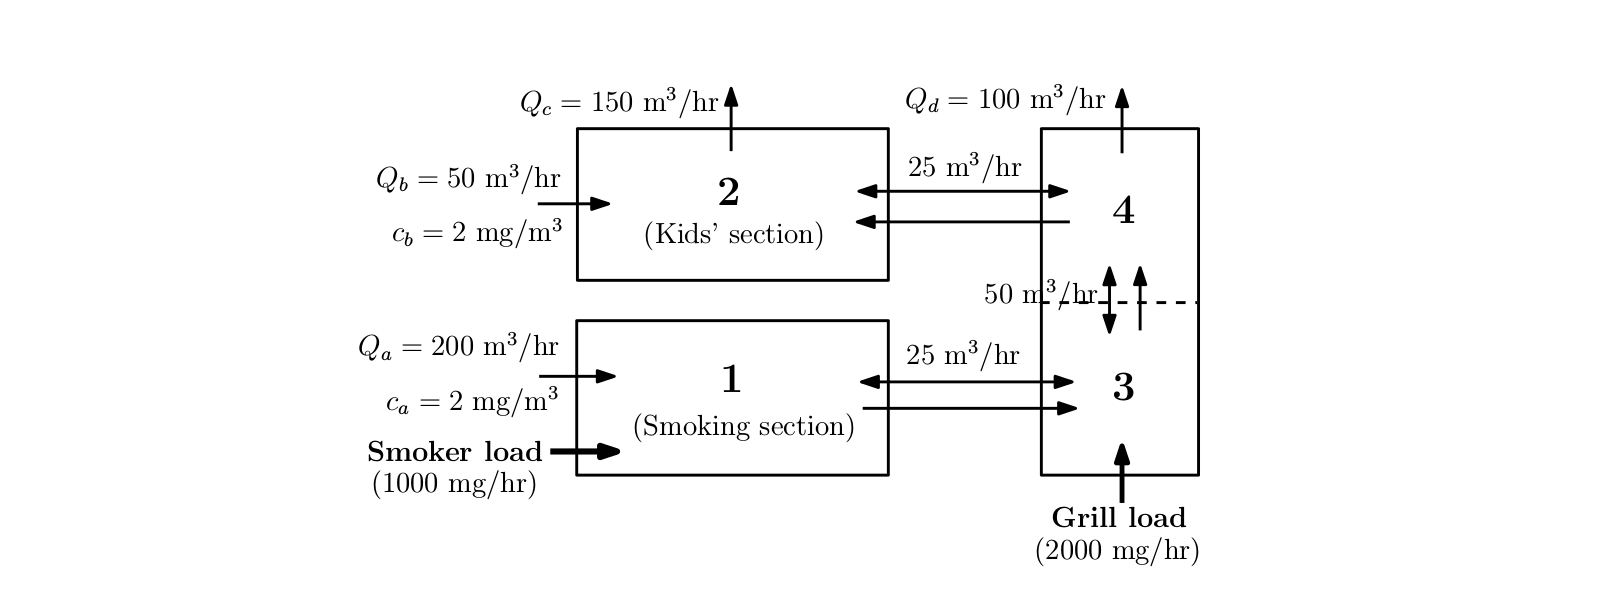
\includegraphics[scale=0.22]{Problem.png}
    
	\subsection{Outline}
	We can model the influx and outflux of \ce{CO2} in each room by using systems of linear equations. Since we know that the rooms are in steady states, the influx of \ce{CO2} must equal the outflux of \ce{CO2} for each of the rooms.
	
	\section{Numerical methods}
	In this section, we will use Gaussian elimination, LU factorization as well as the Jacobian method to solve systems of linear equations.\\
	
	Let ${c1, c2, c3, c4}$ be the concentrations of \ce{CO2} in rooms 1, 2, 3 and 4, respectively. Then from the diagram, we construct the steady-state equations, assuming that outflux must equal influx in the long run:
	
	\[225{\times}c1 + 25{\times}c3 = -1400\]
	\[175{\times}c2 - 125{\times}c4 = 100\]
	\[225{\times}c1 - 275{\times}c3 + 50{\times}c4 = -2000\]
	\[25{\times}c2 + 250{\times}c3 - 275{\times}c4 = 0\]
	
	\section{Results}
    
    \subsection{Using Gaussian elimination}
    Gaussian elimination results in the following:
    ${c1 = 8.0996 mg/m^3}$, ${c2 = 12.3448 mg/m^3}$, ${c3 = 16.8966 mg/m^3}$, and ${c4 = 16.4828 mg/m^3}$
    \subsection{Using LU Factorization}
    The built-in LU factorization method in Matlab results in the exact same results:
    ${c1 = 8.0996 mg/m^3}$, ${c2 = 12.3448 mg/m^3}$, ${c3 = 16.8966 mg/m^3}$, and ${c4 = 16.4828 mg/m^3}$
    \subsection{Using Jacobi method}
    The Jacobi method requires that the matrix must be strictly diagonally dominant in order for the method to converge. Luckily, our matrix satisfies this requirement. Using the initial guesses where all concentrations are ${1 mg/m^3}$, the method converges after 24 iterations, with tolerance ${10^{-6}}$. The results are  ${c1 = 8.0996 mg/m^3}$, ${c2 = 12.3448 mg/m^3}$, ${c3 = 16.8965 mg/m^3}$, and ${c4 = 16.4827 mg/m^3}$
    \subsection{Discussion}
    
    Quite surprisingly, room 1, the designated smoker's room, actually has the lowest concentration of \ce{CO2}. However upon closer inspection, we see that room 1 is very well ventilated, with the outflux measured in ${225 \times c1}$. Room 3 has the highest concentration of \ce{CO2}, because it receives the large outflux of room 1 as parts of its influx. Even though room 3 is quite well ventilated (outflux is measured at ${275 \times c3}$, the heavy influx coming from the grill and from room 1 hold the concentration of \ce{CO2} in this room at a high level.\\
    
    The inverse of the coefficient matrix A is given by Matlab's inv function:
     \[
   		A^{-1}=
  		\left[ {\begin{array}{cccc}
   		0.004996168582375 &  0.000015325670498 & -0.000551724137931 & -0.000107279693487\\
   		0.003448275862069 & 0.006206896551724 & -0.003448275862069 & -0.003448275862069\\
   		0.004965517241379 & 0.000137931034483 & -0.004965517241379 & -0.000965517241379\\
   		0.004827586206897 & 0.000689655172414  & -0.004827586206897 & -0.004827586206897\\
  		\end{array} } \right]
	\]
	Let the constant matrix be \emph{b}, where:
	\[
   		b=
  		\left[ {\begin{array}{c}
   		1400\\
   		100\\
   		-2000\\
   		0\\
  		\end{array} } \right]
	\]
	then we know that the concentration of \ce{CO2} in the second room is precisely the the dot product of the second row of ${A^{-1}}$ and ${b^{T}}$.\\
	As such, the smokers contribute around
	\[\frac{1000}{1400} \times \frac{1400 \times 0.003448275862069}{12.3448} \times 100\% \approx 27.9\%\]
	As for the grills:
	\[\frac{-2000 \times -0.003448275862069}{12.3448} \times 100\% \approx 55.9\%\]
	The rest, ${16.2\%}$, comes from the intake vents.
    \\
    Suppose now smoking is banned, and the grill is fixed. We see that \ce{CO2} contribution in the constant matrix would drop to 400 for the first entry, and 0 for the third. Using Matlab to solve with a new constant matrix, we obtain that the concentration is ${2 mg/m^3}$ for every room.
    \\
    Now suppose that the mixing between areas 2 and 4 is decreased to ${5m^3/hr}$. Then we have a new system:
    \[225{\times}c1 + 25{\times}c3 = -1400\]
	\[155{\times}c2 - 105{\times}c4 = 100\]
	\[225{\times}c1 - 275{\times}c3 + 50{\times}c4 = -2000\]
	\[5{\times}c2 + 250{\times}c3 - 255{\times}c4 = 0\]
	
	The concentration in room 2 drops to 12.0800, which makes sense since room 2 is getting its \ce{CO2} intake from the air circulating in the other 3 rooms. Decreasing the amount of air flowing between 2 and 4 would help reduce the concentration in room 2. However the drop is not too significant since from room 4, there is still a significant portion of volumetric airflow flowing into room 2 at ${100m^3/h}$.
    \section{Appendix for this chapter}
    \subsection{Code for the Gaussian elimination method}
	\lstinputlisting{GE.m}
    \subsection{Code for the Jacobi method}
	\lstinputlisting{Jacobi.m}
    \subsection{Code for this chapter}
	\lstinputlisting{Project3.m}
    
    \chapter{Curve fitting - Cubic spline interpolation}
    \section{Introduction}
    The final part of this book deals with curve fitting given different data points. We switch gear from finding solutions to given equations/systems. and now we do something that is of the opposite nature. Given the data points, we construct a curve that interpolates the data points, giving us a picture of what might have been the equation that gave rise to those data points. The specific technique that we are talking about is cubic spline interpolation. 
    \section{Method explanation}
    By employing cubic curves to fit the intervals of the data points given, we construct a smooth curve that goes through all the data points that we have, in the hope that this curve will give us good estimations of the other points inside the interval created by the given points. Given n data points, we construct n-1 cubic functions that, put together, give us a smooth curve that can be used for further estimations.
    \section{Method formalization}
    Assume that we are given the N data points ${(x_1, Y_1), (x_2, y_2)...(x_N, y_N)}$, where the ${x_i's}$ are distinct and in increasing order. Then a \textbf{cubic spline} ${S(x)}$ through the data points is a set of cubic polynomials ${S_1, S_2...S_{N-1}}$ satisfying the following properties
    \begin{properties}
    	\item ${S_i(x_i) = y_i}$ and ${S_i(x_{i+1}) = y_{i+1}}$ for ${i = 1, 2,...,N-1}$
        \item ${S'_{i-1}(x_i) = S'_i(x_i)}$ for ${i = 2, 3,...,N-1}$
        \item ${S''_{i-1}(x_i) = S''_i(x_i)}$ for ${i = 2, 3,...,N-1}$
    \end{properties}
    \section{Method discussion}
    The above properties gives us ${3N-5}$ equations, however it is easy to see that we have ${N-1}$ cubic functions, each containing 3 unknowns. Therefore we would need to have ${3N-3}$ equations to solve for all the coefficients. The 2 extra equations usually come from endpoint conditions, There are many endpoint conditions, however the next project deals with natural endpoint conditions, meaning that the second derivatives of the first and last functions at the two outermost points evaluate to 0 for both of them.
    \chapter{Thermocline at Platte Lake}
	\section{Abstract}
	This project investigates the thermocline, which is the horizontal plane separating regions of different temperatures in lakes. By using data, which give the depth of water and the corresponding temperature at that depth, collected at Platte Lake, we use the method of cubic spline interpolation to find a function that gives the water temperature at any given depth. Using this function and its first and second derivatives, we are able to find the position at which the thermocline occurs, and from there we can also calculate the heat flux across this thermocline.
	
	\section{Introduction}
	
	\subsection{Background information}
	In this section, we explore the method of cubic spline interpolation, which we will use to interpolate data points collected by experimentation. The data given, reflecting the various water depths and the corresponding water temperature, are collected from Platte Lake.
	
	\subsection{Problem description}
	The first task in this problem is to find a function that models water temperature with respect to changing water depths. After that, we need to find the position of the thermocline. The thermocline is defined to be the point of inflection for the temperature depth graph. In other words, this is the point where ${\frac{d^2T}{dx^2} = 0}$, where T is the temperature, measured in Celcius degrees, and x is the depth, measured in meters. Also, the thermocline is the position at which the absolute value of the first derivative of the graph is at maximum.\\
	After finding the thermocline, we determine the heat flux across the thermocline by using this equation:
	\[J = -\alpha \times \rho \times C \times \frac{dT}{dx}\]
	where ${J}$ is the heat flux in ${cal/(cm^2s}$, ${\alpha}$ is the eddy diffusion coefficient ${cm^2/s}$, ${\rho}$ is the density of water(${\approx 1 g/cm^3)}$, and ${C}$ is the specific heat of water ${\approx 1 cal/gC}$.
    
	\subsection{Outline}
	Here the method chosen to find such a function is the method of cubic spline interpolation. Since this method introduces ${3N - 3}$ unknowns, but we can only construct ${3N - 5}$ linear equations using the properties discussed in class, we have to supply ${2}$ more equations in order to find all the unknowns. The problem wants to explore natural cubic spline interpolation, meaning that if ${f(x)}$ is our function, then ${f''(x) = 0}$ at both of the outermost data points.
	
	\section{Numerical methods}
	In this project, we use the method of cubic spline interpolation, with natural endpoint conditions. Given the data points ${(x1, y1), (x2, y2), ... (xN, yN)}$, the method constructs a function that interpolates all the data points. The code to implement this is attached in the appendix.
	
	\section{Results}
    
    \subsection{Graph of temperature against depth}
    This is the graph produced by using Matlab to construct the cubic spline that interpolates all the data points given:\\
    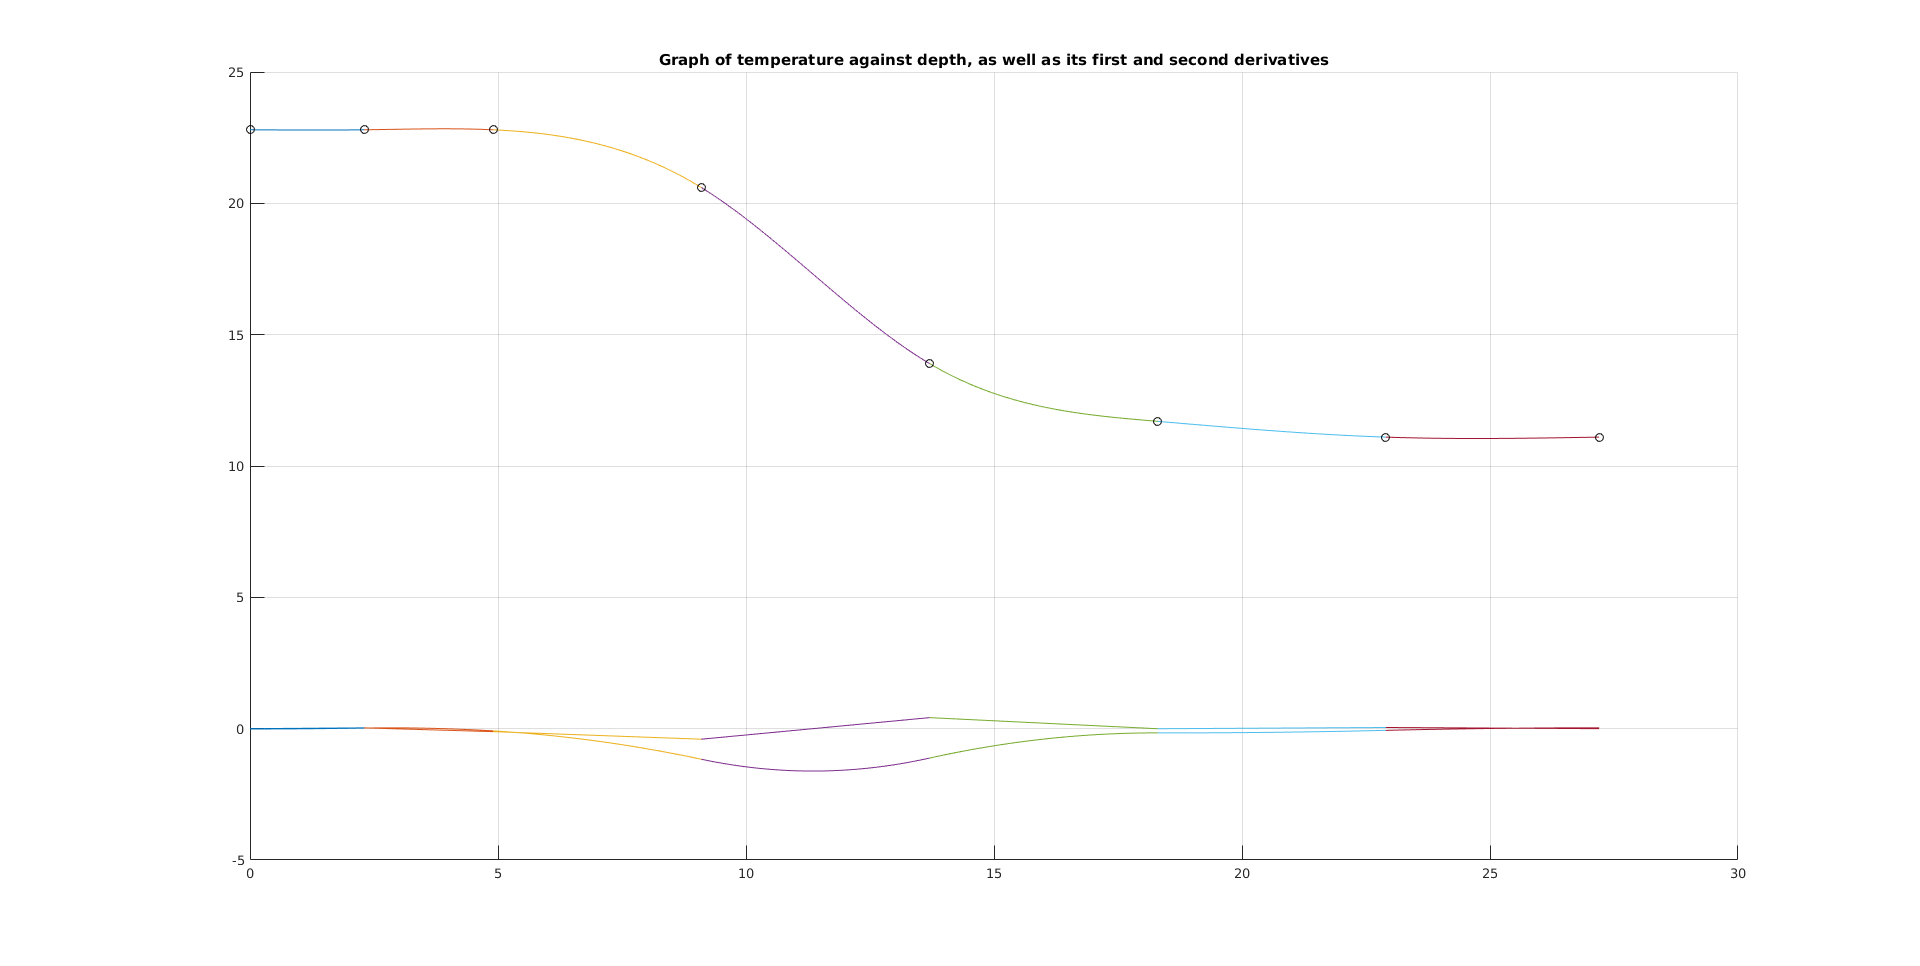
\includegraphics[scale=0.25]{Graph.png}
    \subsection{Discussion}
    From the graph given, we see that the thermocline occurs in the depth between the 4th and the 5th data points, or in the purple cubic function. We proceed to find the function modeling the temperature against depth between those 2 points using the coefficients calculated from before. The, we take the second derivative of that function with respect to the depth. After that, we use the bisection method to find the root of the second derivative in this interval, to give that the thermocline is ${\approx 11.3463673830}$. Plugging this into the equation for the heat flux, we find that the heat flux around the thermocline is ${J\approx1.614055517555187e-04}$
    \section{Appendix for this chapter}
    \subsection{Code for this chapter}
    \lstinputlisting{Project4.m}
    \subsection{Natural Cubic Spline calculation in Matlab}
    \lstinputlisting{spline_natural.m}
\end{document}

\end{document}